% Drawing 156-3/02-1 -- folder 156-3, batch 02, archive page 23 (PDF page 24).
% Transcription: en marge gauche, une bande oblique hachurée, coupée transversalement par quatre arcs épais marqués (de haut en bas) $y$, $b$, $a$, $x$ ; la partie entre $b$ et $a$ plus fortement hachurée, les arcs $a$ et $x$ partant d'un même point du bord gauche.
% Kind: hatched band cut by four arcs (a « faille »). Method 2 (schematic redraw from the facsimile). Status: ok.
% Notes: A long oblique band (two straight sides, a faint cap at each end, the right side running a little past the lower cap as on the page), cut across by four thick arcs, all ending on the sides at computed points: y at the top, then b, then a; the arc x leaves the left side at the same computed point as a and curves down to the right side. The part between b and a is densely hatched (drawn as a hatched region); the light hatching elsewhere is drawn as a few pencil strokes at approximately their places, not stroke for stroke. Labels as on the page: y on both sides of its arc, b at the left and a glyph read b at the right of its arc, a at the left (above x) and at the right of its arc, x at the left and at the lower end of its arc. Doubtful: the glyph at the right of the second arc (read b, could be a), and the lower label of x. Nothing struck. Redrawn 2026-11-09 (issue 128): to check again. Question settled by a machine pass on the facsimile, 2026-11-12 (maths): each arc carries its letter at both ends (y and y, a and a, x and x), so the glyph at the right end of the second arc is b and the lower label of the last arc is x, as drawn. Not checked by a reader. 2026-11-13, Claude Opus 5.5, overlay check (issue 147): not compiled (no TeX in the session); the TikZ rasterised and laid over the 350 dpi colour render of the scan, with ink/pencil separations of the crop. Redrawn on the ink: the sides of the band as the slightly bent lines they are; the top of the band is not a cap joining the sides but the first of the hatching strokes (it touches neither side), and the lower end is closed by a pencil stroke from the left corner only, running on past the right side's line; the four arcs through points read on them (b was 1.5 units low); the hatching stroke for stroke instead of a pattern and a few strokes at approximate places: above b, eight strokes (five in ink, three in pencil), between b and a the eleven heavy strokes of the dense hatching, below a and x six faint pencil strokes, two of them broken; the eight labels on their glyphs. Every element lies on the ink to within about 1 unit.
% Coordinates: 1 unit = 1 mm = 1/100 of the crop width (bbox in page fractions: [0.08, 0.61, 0.21, 0.78]).
% Redrawn by Claude (claude-opus-5-5), issue #73, 2026-11-09; not checked by a human; not compiled (no TeX in the session).
% Revised by Claude Opus 5.5 (claude-opus-5-5), issue #147, 2026-11-13: overlay check on the colour scan; not checked by a human; not compiled (no TeX in the session).
% Rights: reproduces part of the work -- behind RENDER_TRANSCRIPTS, never published by itself.
\documentclass[tikz,border=3pt]{standalone}
\usepackage{amsmath,amssymb}
\usetikzlibrary{patterns,arrows.meta}
\tikzset{pencil/.style={black!45}, struck/.style={black!35}, mark/.style={circle,draw,inner sep=1.3pt}, pt/.style={circle,fill,inner sep=0.9pt}, opt/.style={circle,draw,fill=white,inner sep=1.1pt}}
\begin{document}
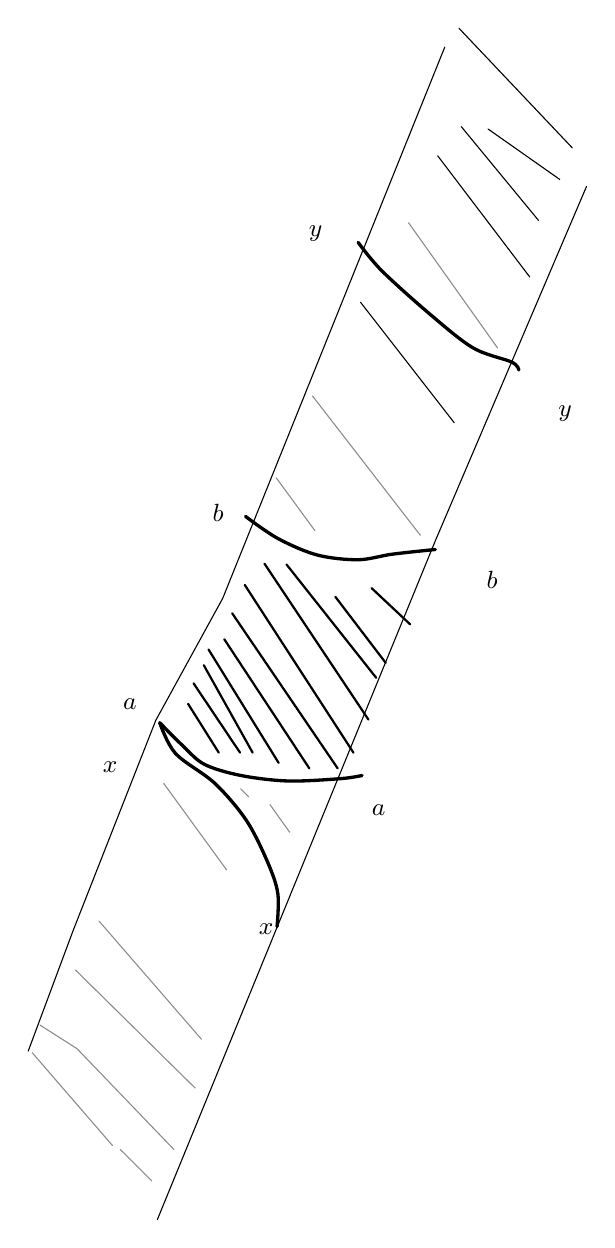
\begin{tikzpicture}[x=1mm,y=1mm,line cap=round,line join=round,font=\scriptsize]
% the two sides of the band
\draw (71.2,-19.8) -- (43,-89.8) -- (34.5,-105.3) -- (24,-132) -- (18.3,-147.3);
\draw (89.2,-37.5) -- (70,-82.5) -- (34.7,-168.7);
% the pencil stroke closing the lower end
\draw[pencil] (18.8,-147.5) -- (29,-159.3);
% the four thick arcs y, b, a, x
\draw[very thick] plot[smooth, tension=0.55] coordinates {(60.2,-44.6) (63.2,-48.2) (69.3,-53.7) (74.8,-58) (79.7,-59.8) (80.6,-60.8)};
\draw[very thick] plot[smooth, tension=0.55] coordinates {(45.9,-79.4) (50,-82.2) (55,-84.3) (60.2,-84.9) (64.5,-84.2) (70,-83.6)};
\draw[very thick] plot[smooth, tension=0.55] coordinates {(35,-105.6) (38,-108.6) (40.7,-110.9) (45.3,-112.3) (51.3,-113) (58,-112.7) (60.7,-112.3)};
\draw[very thick] plot[smooth, tension=0.55] coordinates {(35,-105.6) (37,-109.5) (42,-113.3) (46,-118) (48.7,-123.3) (50,-127.3) (49.9,-131.5)};
% light hatching above b (ink, and pencil where so)
\draw (73,-17.4) -- (87.4,-32.6);
\draw (76.7,-30.2) -- (85.8,-36.6);
\draw (73.3,-29.9) -- (83.1,-41.8);
\draw (70.3,-33.6) -- (82,-49);
\draw[pencil] (66.6,-42.1) -- (77.9,-58);
\draw (60.5,-52.2) -- (72.4,-67.5);
\draw[pencil] (54.4,-64.1) -- (68.1,-81.8);
\draw[pencil] (49.8,-74.5) -- (54.7,-81.2);
% dense hatching between b and a, stroke by stroke
\draw[thick] (48.3,-85.4) -- (61.5,-105.2);
\draw[thick] (51.1,-85.5) -- (62.5,-99.9);
\draw[thick] (57.3,-89.6) -- (63.7,-98);
\draw[thick] (61.9,-88.5) -- (66.8,-93.1);
\draw[thick] (45.8,-88.1) -- (59.6,-109.4);
\draw[thick] (44.2,-91.7) -- (57.6,-111.4);
\draw[thick] (43.2,-95) -- (54,-111.4);
\draw[thick] (41.2,-96.3) -- (50.1,-110.7);
\draw[thick] (40.6,-98.3) -- (46.8,-109.4);
\draw[thick] (39.3,-100.6) -- (45.2,-109.4);
\draw[thick] (38.6,-103.2) -- (42.5,-109.4);
% light pencil hatching below a and x
\draw[pencil] (35.5,-113.3) -- (43.5,-124.3);
\draw[pencil] (45.3,-114) -- (46.3,-115);
\draw[pencil] (49,-116) -- (51.5,-119.5);
\draw[pencil] (27.3,-130.8) -- (40.3,-145.8);
\draw[pencil] (24.3,-137) -- (39.5,-152);
\draw[pencil] (19.8,-144) -- (24.5,-147) -- (36.8,-159.8);
\draw[pencil] (30,-159.8) -- (34,-163.8);
% labels: each arc carries its letter at both ends
\node[inner sep=1pt] at (54.8,-43.5) {\small $y$};
\node[inner sep=1pt] at (86.5,-66.4) {\small $y$};
\node[inner sep=1pt] at (42.4,-79) {\small $b$};
\node[inner sep=1pt] at (77.2,-87.4) {\small $b$};
\node[inner sep=1pt] at (31.2,-103.3) {\small $a$};
\node[inner sep=1pt] at (62.8,-116.7) {\small $a$};
\node[inner sep=1pt] at (28.7,-111.2) {\small $x$};
\node[inner sep=1pt] at (48.5,-131.8) {\small $x$};
\end{tikzpicture}
\end{document}
